\documentclass[10pt]{article}
\usepackage[polish]{babel}
\usepackage[utf8]{inputenc}
\usepackage[T1]{fontenc}
\usepackage{amsmath}
\usepackage{amsfonts}
\usepackage{amssymb}
\usepackage[version=4]{mhchem}
\usepackage{stmaryrd}
\usepackage{graphicx}
\usepackage[export]{adjustbox}
\graphicspath{ {./images/} }

\title{LIGA MATEMATYCZNA \\
 im. Zdzisława Matuskiego \\
 LISTOPAD 2017 \\
 GIMNAZJUM }

\author{}
\date{}


\begin{document}
\maketitle
\section*{ZADANIE 1.}
O liczbach \(a, b, c, d\) wiadomo, \(\dot{z}\) e

\[
\left\{\begin{array}{l}
a=b c d \\
a+b=c d \\
a+b+c=d \\
a+b+c+d=1
\end{array}\right.
\]

Wyznacz te liczby.

\section*{ZADANIE 2.}
Niech \(p\) będzie liczbą pierwszą taką, że liczba dzielników liczby \(p^{6}\) jest dzielnikiem tej liczby. Ile dzielników ma liczba \((p+1)^{6}\) ?

\section*{ZADANIE 3.}
Dziadek Ani urodził się przed II wojną światową, ale ma mniej niż 90 lat. Gdy w 2007 roku obchodził urodziny, Ania zauważyła, że numer roku był równy numerowi roku urodzenia dziadka powiększonemu o pięciokrotną sumę cyfr roku urodzenia. W którym roku urodził się dziadek Ani?

\section*{ZADANIE 4.}
Dwa jednakowe koła mniejsze i jedno koło większe wpisano w prostokąt w taki sposób, że koła są styczne do boków prostokąta i wzajemnie styczne zewnętrznie. Mniejszy z boków prostokąta ma długość 4 . Oblicz obwód prostokąta oraz różnicę między polem prostokąta a sumą pól kół.\\
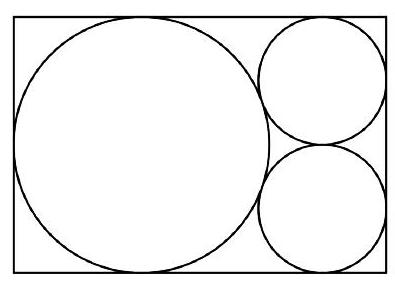
\includegraphics[max width=\textwidth, center]{2024_11_21_7bef91178e532250cdc3g-1}

\section*{ZADANIE 5.}
Wykaż, że liczba \(4^{202}+2 \cdot 4^{101} \cdot 6^{101}+6^{202}\) jest podzielna przez 100 .


\end{document}